\documentclass[11pt]{article}
%\usepackage[authoryear, square]{natbib}
\usepackage{mathptmx}
%\usepackage{eucal}
\usepackage{amsmath}
\usepackage{amscd}
\usepackage{amssymb}
\usepackage{amsthm}
\usepackage{xspace}
\usepackage[all,tips]{xy}
\usepackage[dvips]{graphicx}
\usepackage{verbatim}
\usepackage{syntonly}
\usepackage{hyperref}
\usepackage{graphics,fullpage,color, epsfig,url}
\usepackage{multirow,array}
%\usepackage{cite}
%\renewcommand{\refname}{\vskip -20 pt}
\usepackage{setspace}
\setstretch{1.2}
\usepackage{fontspec}
\setmainfont{Arial}

\usepackage{lastpage}
\usepackage{ifthen}
\usepackage{fancyhdr}

\usepackage{stmaryrd}
\usepackage{multirow,mathtools,latexsym, mathrsfs, pdftricks,framed,listings,mleftright}

\pagestyle{fancy}
\fancyhf{}
\renewcommand{\headrulewidth}{0pt}
\renewcommand{\footrulewidth}{0pt}
\fancyfoot[C]{\ifthenelse{\thepage=\pageref{LastPage}}{}{\thepage}}
\fancyfoot[L]{}


\theoremstyle{plain}% default
\newtheorem{prototheorem}{Theorem}


\newtheorem{theorem}[prototheorem]{Theorem}
\newtheorem{lemma}[prototheorem]{Lemma}
\newtheorem{proposition}[prototheorem]{Proposition}
\newtheorem{corollary}[prototheorem]{Corollary}
%\newtheorem{definition}[prototheorem]{Definition}
%\newtheorem{remark}[prototheorem]{Remark}
\newtheorem{example}[prototheorem]{Example}



\newtheorem{algorithm3}{Algorithm}


\providecommand{\bysame}{\leavevmode\hbox to3em{\hrulefill}\thinspace}
\providecommand{\MR}{\relax\ifhmode\unskip\space\fi MR }
% \MRhref is called by the amsart/book/proc definition of \MR.
\providecommand{\MRhref}[2]{%
  \href{http://www.ams.org/mathscinet-getitem?mr=#1}{#2}
}
\providecommand{\href}[2]{#2}

%%%%%%%%%%%%%%%%%%%%%%%%%%%%%%%%%%%%%%%%%%%%%%%%%%%%%%%%%%%%%%%%%%%%%%%%%
%%%%%%%%%% EXACT 1in MARGINS %%%%%%%                                   %%
\setlength{\textwidth}{6.5in}     %%                                   %%
\setlength{\oddsidemargin}{0in}   %% (It is recommended that you       %%
\setlength{\evensidemargin}{0in}  %%  not change these parameters,     %%
\setlength{\textheight}{8.5in}    %%  at the risk of having your       %%
\setlength{\topmargin}{0in}       %%  proposal dismissed on the basis  %%
\setlength{\headheight}{0in}      %%  of incorrect formatting!!!)      %%
\setlength{\headsep}{0in}         %%                                   %%
\setlength{\footskip}{.5in}       %%                                   %%
%%%%%%%%%%%%%%%%%%%%%%%%%%%%%%%%%%%%                                   %%
\newcommand{\required}[1]{\section*{\hfil #1\hfil}}                    %%
%\renewcommand{\refname}{\hfil Refe\hfil}                   %%
%%%%%%%%%%%%%%%%%%%%%%%%%%%%%%%%%%%%%%%%%%%%%%%%%%%%%%%%%%%%%%%%%%%%%%%%%
\DeclarePairedDelimiterX{\distx}[2]{(}{)}{%
  #1  ,  #2%
}
\newcommand{\TV}{\mathrm{TV}\distx}
\newcommand{\lb}[1]{{\lfloor #1 \rfloor}}
\newcommand{\ub}[1]{{\lceil #1 \rceil}}
\def\spanset{\operatorname{span}}




\definecolor{gray_color}{rgb}{0.508787,0.506616,0.454318}
\definecolor{gold_color}{rgb}{0.973141,0.682118,0.039365}
\definecolor{blue_color}{rgb}{0.049179,0.249936,0.564133}

\newcommand{\resp}[1]{{{\it \color{gray_color} #1}}} % Important points/questions


\usepackage[backend=biber,backref=true,style=numeric,firstinits=true,maxbibnames=9]{biblatex}
\addbibresource{nawaf.bib}

\begin{document}

\pagestyle{empty} 

\section*{Delayed Rejection for Adaptive-Step-Size Hamiltonian MCMC}

Nawaf Bou-Rabee (Rutgers) \& Bob Carpenter (Flatiron) 

\section*{Summary of Work}

This note presents a potential issue with the delayed rejection algorithm for adapting the time step size in the numerical integration of the Hamiltonian flow underlying Hamiltonian MCMC methods (e.g. Hamiltonian Monte Carlo, generalized Hamiltonian Monte Carlo, randomized Hamilonian Monte Carlo, etc.).   The delayed rejection algorithm is a generalization of the Metropolis-Hastings algorithm that allows for multiple proposal distributions within each transition step \cite{mira2001metropolis,green2001delayed}.  As the name suggests, the idea is to use draws from some other proposal distributions in case of rejection, and thereby, delay  rejection.  For generalized Hamiltonian Monte Carlo, this idea has recently been proposed for `extra chances' \cite{campos2015extra} and `adaptive step size selection' \cite{ChBaCa2023}.  Here we prove two things about the latter approach: \begin{itemize}
\item If the first proposal move is inexact and the second proposal move is exact, then the acceptance probability of the second proposal move is not equal to unity.  (See Lemma~\ref{lem:exactsecond} below.)
\item Moreover, if the subsequent proposal moves are all exact, then the acceptance probability of the subsequent proposal moves is identically zero.  (See Lemma~\ref{lem:exactinfinite} below.)
\end{itemize}
In other words, the first proposal move affects (or pollutes?, or contaminates?) \emph{all} subsequent proposal moves even when these proposal moves are exact.  Importantly, refining the time step size may not (as one would hope) improve the acceptance probability for subsequent proposal moves.  In addition to  Lemma~\ref{lem:exactsecond} and Lemma~\ref{lem:exactinfinite} below, simple  verification is provided in the context of a standard normal target distribution and Verlet time integration.   

\section*{Motivation}

Why are we interested in delayed rejection for adaptive-step-size HMC?  In practice, adaptive-step-size selection has the potential for more efficient numerical integration of the Hamiltonian flow underlying Hamiltonian MCMC. (In fact, Leslie Greengard asked about adaptive step size selection for Hamiltonian Monte Carlo during a CCM colloquium by Bob Carpenter.)  In terms of theory, it would fit the growing body of literature which deduce convergence results for implementable Hamiltonian MCMC chains by careful comparison to a corresponding non-implementable Hamiltonian MCMC chain that uses the exact solution of a Hamiltonian ODE; see, e.g.,  \cite{BouRabeeOberdoerster2023}.  However, this comparison argument requires a sufficiently high acceptance rate, which might be computationally expensive to attain with constant time step size.



\section*{Delayed Rejection}

We more or less follow the nicely written description given in \cite{ChBaCa2023}. 
Let $\mathcal{M}:  \mathbb{R}^{2d} \to  \mathbb{R}^{2d}$ be the velocity flip involution.  Let $\pi: \mathbb{R}^{2d} \to \mathbb{R}$ denote a density of the target distribution (in phase space) up to a normalization constant, which for simplicity we assume has the form \begin{equation} \label{eq:target}
\pi(z) = e^{-H(z)} \;, 
\end{equation} where $H: \mathbb{R}^{2d} \to \mathbb{R}$ is a Hamiltonian function that satisfies $H \circ \mathcal{M} \equiv H$. 
 Given a collection of $k$  volume-preserving involutions $\{ F_i \}_{i=1}^k$, the transition kernel $\Theta$ of the delayed rejection step  can be written as \begin{equation}
\Theta(z, dz') = \sum_{i=1}^k \tilde{\alpha}_i(z) \prod_{j=1}^{i-1} (1-\tilde{\alpha}_j(z)) \delta_{F_i(z)}(dz') + r(z) \delta_{z}(dz')
\end{equation}
where $r(z) = \prod_{j=1}^k (1-\tilde \alpha_j(z))$, and remarkably, for any $i \in \{ 1, \cdots, k \}$, the $i$-th acceptance probability function is given by the following clever recurrence relation: \begin{equation} \label{eq:recurrence}
\tilde \alpha_i (z) = \min\left(1, \dfrac{\pi(z') \prod_{j=1}^{i-1} (1- \tilde \alpha_j(z'))}{\pi(z) \prod_{j=1}^{i-1} (1- \tilde \alpha_j(z))} \right) \;,  \quad \text{where} \quad z' = F_i(z) \;.
\end{equation}
To be sure, the initial condition of this recurrence relation is the usual Metropolis-Hastings ratio, i.e.,  $\tilde \alpha_1 (z) = \min(1, \pi\circ F_1(z))/\pi(z))$.  

  


\section*{Main Findings}

By evaluating \eqref{eq:recurrence} at $i=2$, and simplifying under the assumption that $F_2$ is exact (i.e., $H \circ F_2 \equiv H$), we obtain the following finding.

\begin{lemma} \label{lem:exactsecond}
Let $z \in \mathbb{R}^{2d}$ be such that  $\tilde{\alpha}_1(z) < 1$, i.e., $\pi \circ F_1(z) < \pi(z)$.  Moreover, suppose that the second volume-preserving involution satisfies $H \circ F_2 \equiv H$ (i.e., $F_2$ is exact).  Then \begin{equation} \label{recurrence_i_eq_2_exact}
\tilde{\alpha}_2(z) = \min\left(1, \dfrac{  (\pi(z)  -  \pi \circ F_1 \circ F_2(z) )^+ }{  \pi(z) - \pi \circ F_1(z) } \right) \;.
\end{equation}
\end{lemma}

From \eqref{recurrence_i_eq_2_exact}, note that $\tilde{\alpha}_2(z)$ is not equal to unity in general.  


\medskip


Now, suppose the second proposal is also rejected. Does it help to take more exact proposals?  Unfortunately, not.  


\begin{lemma} \label{lem:exactinfinite}
    In the situation of Lemma~\ref{lem:exactsecond}, suppose further that $\tilde{\alpha}_2(z) < 1$, i.e., $ \pi(z) - \pi \circ F_1(z) > \pi(z) - \pi \circ F_1 \circ F_2 (z)$.  Moreover, suppose that the subsequent volume-preserving involutions satisfy $H \circ F_i \equiv H$ for all $i \in \mathbb{N}$ such that $i>2$. Then, for all $i>2$, $\tilde{\alpha}_i(z) = 0$.  
\end{lemma}

\begin{proof} This lemma is straightforward to prove by induction.  

\medskip

For the base case ($i=3$), \[
\tilde \alpha_{3} (z) = \min\left(1, \frac{ (1- \tilde \alpha_1 \circ F_2(z)) (1- \tilde \alpha_2 \circ F_2(z))}{(1- \tilde \alpha_1(z)) (1- \tilde \alpha_2(z))} \right) = 0 \;. 
\] Since $\pi(z) - \pi \circ F_1(z) > \pi(z) - \pi \circ F_1 \circ F_2(z) $,  \[
\tilde \alpha_2 \circ F_2(z) = \min\left( 1 , \dfrac{\pi(z) - \pi \circ F_1(z)}{\pi(z) - \pi \circ F_1 \circ F_2(z)} \right) = 1 \;,
\] and hence, $\tilde{\alpha}_3 (z) = 0$.   

\medskip

For the induction hypothesis, suppose that $\tilde{\alpha}_i(z)=0$ for $i \in \{3, \cdots, n \}$ , then from \eqref{recurrence_i_eq_2_exact}, \[
\tilde \alpha_{n+1} (z) = \min\left(1, \frac{\prod_{j=1}^{n} (1- \tilde \alpha_j \circ F_2(z) )}{(1- \tilde \alpha_1(z)) (1- \tilde \alpha_2(z))} \right) = 0 \;.
\] Since $\pi(z) - \pi \circ F_1(z) > \pi(z) - \pi \circ F_1 \circ F_2(z) $, we again have $\tilde \alpha_2 \circ F_2(z) = 1$, and hence, $\tilde{\alpha}_{n+1} (z) = 0$.  
\end{proof}

\section*{Illustration}


Suppose that $\pi(x) = e^{-x^2 / 2}$, i.e., the target distribution is standard normal.  Let $F_1 = \mathcal{M} \circ \theta_{h}$ where $\theta_h: \mathbb{R}^{2d} \to \mathbb{R}^{2d}$ is one step of velocity Verlet operated with time step size $h>0$.  In this case, it is easy to show that velocity Verlet preserves a modified Hamiltonian $H_h(z)$ such that $H(z) = H_h(z) + \frac{1}{8} h^2 |x|^2$ where $z=(x,v) \in \mathbb{R}^{2d}$; see, e.g., Chapter 5.3 of \cite{BouRabeeEberleLectureNotes2020}. Let $F_2$ denote the exact solution of this Hamiltonian flow at time $h$.  Thanks to the recurrence \eqref{eq:recurrence}, \[
\tilde{\alpha}_2(z) = \min\left(1, \dfrac{1-\tilde{\alpha}_1 \circ F_2(z)}{1-\tilde \alpha_1(z)} \right) \;.
\] For velocity Verlet, it is easy to check that \[
\tilde{\alpha}_1(z) = \exp( - G(x,\tilde{x})^+) \quad \text{where} \quad G(x,\tilde{x}) = \frac{h^2}{8} ( |\tilde{x}|^2 - |x|^2)
\] where $\tilde{z} = (\tilde{x}, \tilde{v})$ and $\tilde{x}(x,v) := (1-h^2/2) x + h v$.   Moreover, the exact solution $z'=(x',v')=F_2(z)$ from $z=(x,v)$ over a duration of length $h$ satisfies $x':=\cos(h) x + \sin(h) v$ and $v':=-\sin(h) x + \cos(h) v$. Hence, \[
\tilde{\alpha}_1 \circ F_2(z) = \exp\left( -G(x',\tilde{x}(x',v'))^+ \right)  \;.
\]  Combining these results and expanding reveals that $\tilde{\alpha}_2(z)  = O(h^3)$, as confirmed in Figure~\ref{fig:alpha2}.

\begin{figure}[ht!] 
\centering
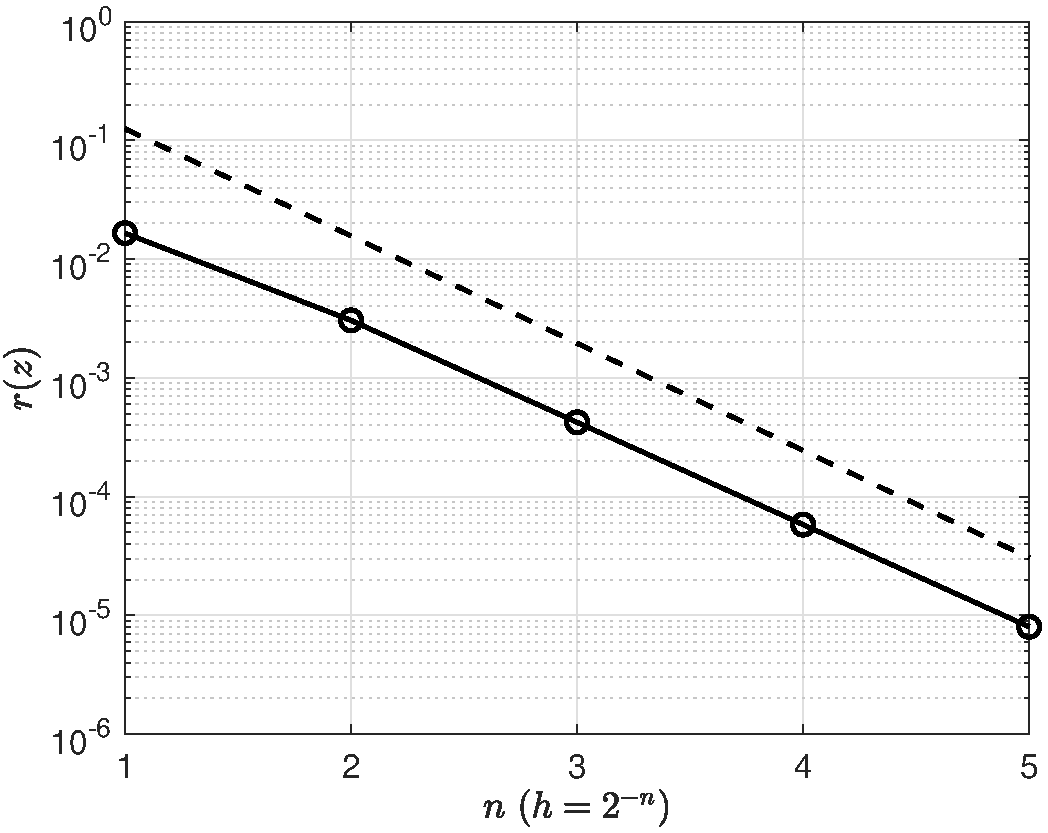
\includegraphics[scale=0.8]{img/alpha2.pdf}
\caption{ A plot of the rejection rate in the delayed rejection algorithm with $k=2$ applied to a standard normal target with Hamiltonian function $H(x,v) = (1/2) (v^2 + x^2)$.  The first proposal move is inexact (given by one step of Verlet operated with time step size $h>0$) while the second proposal move is exact. The initial condition is $x=2$ and $v=1$. The time step sizes tested  are $h=2^{-n}$ where $n$ is given on the horizontal axis. The dashed curve is $h^{3} = (2^{-n})^3$ versus $n$.  }
\label{fig:alpha2}
\end{figure}


\printbibliography

\clearpage


%\vspace{-0.5in}







\end{document}
